
\chapter{Methodology}
\label{chap:new_ideas}


\section{How will we carry out this investigation}

Our research process consists of taking a promising proposal, implement our own system based on the theoretical framework provided, evaluate the result of the query reformulation from this resulting system, and later attempt to improve it's performance.



\section{Overview of Deep learning methods in Information Retrieval}

The use of deep neural networks in information retrieval 

Natural language processing has been a major application of machine learning since the early days, information retrieval is closely related to NLP.






\section{Deep reinforcement learning }



\subsection{Reproducing experiments}

In an exploratory paper, Nogueira \& Cho\cite{nogueira2017task} proposed the idea of incorporating deep reinforcement learning to perform pseudo relevance feedback.  In this thesis we first aim to reproduce the system based on the description from Nogeura and Cho, and check if we get comparable results 


\todo{Discuss why this is non-trivial}


\subsection{Expand}




There are two variants of the model, one uses CNN and one uses RNN, we aim to work with the CNN variant 




We approach the discussion in two parts. The first part covers the theoretical framework which we base our experiments on, the second part describes practical components involved, such as software systems used. 



\section{Nogueira and Cho's framework}

Nogueira \& Cho \cite{nogueira2017task} 's framework poses the problem of query reformulation as a reinforcement learning problem. Where an agent learns to interact with an environment (the search engine) to maximize some reward. This method takes a pseudo relevance feedback approach, assuming the user has a reasonable idea of what they are looking for, and that the original query is somewhat relevant. This method does not account for spelling error or other query errors.

Nogueira \& Cho \cite{nogueira2017task}  stated that the most important implication under this framework was treating the environment as a black box and achieving end to end learning.

The process involves performing an initial round of search using the original query, $q_0$. This retrieves a set of documents, $D_0$ based on the raw query. Terms from $D_0$ are referred to as candidate terms.  A deep reinforcement learning agent is trained to rewrite the query using the set of candidate terms, producing a new query, $q'$. The rewritten query is then sent to the search engine, the results are scored based on relevance assessment to produce a scalar reward, which is returned to the reinforcement learning agent to indicate how successful the reformulation was.  The agent's goal is to maximize this reward.  This means that in principle it is possible to train the agent to perform arbitrary tasks by changing the reward function. 

There were several points of ambiguity we found in the description, which are open to interpretation. When we first began working with this framework it was not entirely clear from the description provided in the paper what the state and action is at each time step. These aspects are crucial to a reinforcement learning problem. We assumed this would be a trivial issue that will become obvious as we progress with implementation. Later on we found this ambiguity to be problematic, a topic we will discuss in the next chapter. 


We use this framework as a starting point in our research, deriving our theoretical framework and implementation based on descriptions provided in the paper. 

Part of our motivation for basing our systems on this framework stems from our interest in exploring the capability of deep reinforcement learning. Another perhaps more important motivation is from the high retrieval performance claimed by this paper, which outperforms baselines such as BM25. As previous literature suggests that there has been little to no improvement on ad-hoc retrieval from the standard BM25 ranking function in the past two decades, we wish to collect further evidence on the subject. 



\missingfigure[]{An abstract diagram of the model}



\section{Components in the theoretical framework}

\subsection{An abstract view}

From a bird's eye view, this framework can be thought of as containing the following component

\begin{itemize}
    \item Term embedding layer
    \item Feature extraction layer 
    \item Prediction layer
\end{itemize}

This architecture is common in neural network for classification



\begin{figure}
  \centering
    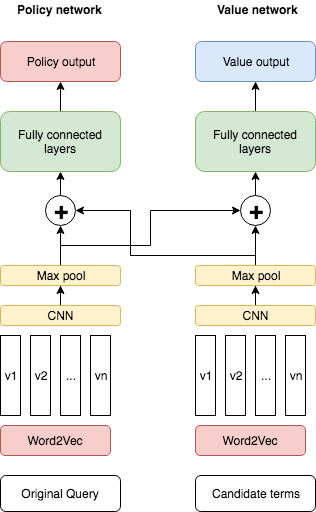
\includegraphics[width=0.5\textwidth]{twonetwork.png}
  \caption{Architecture of our model}
    \label{fig:twonetwork}

\end{figure}

As figure \ref{fig:twonetwork} shows, there are 



\subsection{Word embedding layer}

\subsubsection{Role in our system}


A word embedding layer can be viewed as a form of data pre-processing in the context of machine learning. The word embedding layer need to provide several purposes in the system. 

The first is to build features by representing raw natural language terms as numeric features, such that tokens in the English language can be processed by a software system. 

Secondly, the features should be relatively dense for more efficient learning.  

Thirdly, as the query reformulation problem requires rewriting a query with terms similar to the original query, natural language terms with similar semantic should have their similarity preserved. 

For this reason we used Word2Vec,a neural network based word embedding technique introduced by Mikolov et al.\cite{mikolov2013distributed}. It is a popular word embedding scheme used in information retrieval and natural language processing tasks. 

This technique has several interesting properties which contributes to it's popularity.  Firstly, the model embeds terms into a low dimensional vector space that captures the semantic relationships between words in their vector representation, this is based on the Distribution Hypothesis (CITE), which suggests that terms that appear in close proximity with each other are likely to be related either semantically or syntactically. The most commonly cited example being "King – Man = Queen" as mentioned by Mikolov et al in their work. Capturing the semantic relationship between terms is very useful for natural language processing tasks such as topic clustering and sentence generation.  

\subsubsection{Training a word2vec model}

Word2vec use a three layer shallow neural network trained with self-supervised learning. There are two variants of Word2Vec model, Continuous Bag Of Word (CBOW) model, and Skip-gram. In the CBOW variant, the model takes a one-hot representation (make sure to explain this in background chapter) of a set of terms as inputs to the neural network. These input terms are projected to neurons in the hidden layer. This is then connected to the output layer where each output is the probability of the next term in the sentence given the context terms, computed through a softmax activation function.  


\todo{loss formula and other maths here}

The ground truth is the next term in the sentence, and the prediction error is back propagated through the network to update weights. This requires no human labelling, hence why it is a self supervised learning method. The skip gram variant of Word2vec is very similar to CBOW, the only difference is the model is predicting the context terms given a target term.  CBOW is commonly agreed to be faster, while skip gram is slower to train, but better for infrequent words. 

 
\subsubsection{Hidden layer weight as embedding}

After training completes, the output layer is discarded, the weights in the hidden layer of the model is the word embeddings ready to be used. 
% Explain this some more. Weight matrix stuff 

When training the Word2vec embedding scheme,the number of desired dimensions for the term vectors is a parameter that can be custom defined. There is no common consensus on the suitable number of dimensions to use, as it is a heuristics dependent on the size of the corpus used for training. Common range used by others in the Natural Language Processing community range from 50 to 500 dimensions.  







\subsection{Convolutional Neural Network for text processing}

Once dense representation of terms are acquired through the term embedding scheme, the next part of the system involves passing this input data to a convolutional neural network to extract useful features. The framework outlined by Nogueira \& Cho \cite{nogueira2017task} provided limit information on the use of convolutional neural network. The only mentioning of CNN in the paper is that CNN followed by max pooling was used to obtain a fixed size vector representation for the query and the candidate terms. 


We build our CNN module using an approach that is most commonly used for natural language processing tasks, outlined by Kim(2014) \cite{kim2014convolutional} originally for the purpose of text classification, which builds on a previous approach by Collobert et al \cite{collobert2011natural}. This approach is inspired by the use of CNN in image processing, but contains several point of important difference. Firstly,image based tasks involves the use of 2D image in the RGB space. The convolution filter convolve over these dimensions and extract features. In text processing, there is only dimension per word (in vector format). One term is represented by a 1 dimensional vector. A phrase or a sentence is represented by a concatenation of $K$ * number of embedding dimensions. 


Secondly, CNN architecture used by image based tasks is often hierarchical. Max pooling is used to down sample the features extracted in previous layers in a spatial manner. Our model differs from this approach by using filters of various sizes.


a convention known as "max over time pooling". This means that the max along the time dimension is taken as the representation for the input vectors. 

The input to the CNN layer are a set of words, a phrase (either a query, or some candidate terms) embedded by Word2Vec, concatenated together into a matrix

\begin{equation}
{\mathbf{X} = \mathbf{x}_1 \oplus \mathbf{x}_2\oplus \mathbf{x}_3 ... \oplus \mathbf{x}_n}
\end{equation}

Where $\mathbf{x} \in \mathbb{R}^m $ and $n$ is the size of the input text and $m$ is the number of dimensions chosen to represent a term under the term embedding scheme. This is conceptually similar to an input image in the case of convolutional neural network for computer vision. $n$ and $m$ can be viewed as equivalent to the width and height of the image. Figure \ref{fig:cnn_1} provides a graphical illustration of the input to the CNN. 

\begin{figure}

  \centering
    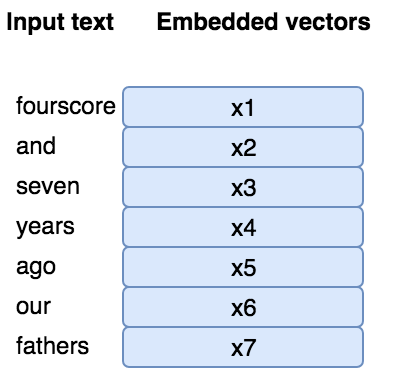
\includegraphics[width=0.5\textwidth]{images/chpt_3/cnn_1.png}
  \caption{An illustration of the input to the CNN}
    \label{fig:cnn_1}

\end{figure}


From this input, feature maps are generated by convolutional filters, also commonly referred to as kernels in literature. A filter is a weight vector 

For image based application of CNN, this involves moving the filter through each region of the image along the width and height dimension to capture features at each point.

However for text input data, this filter only moves in one dimension, and the 


$\mathbf{w} \in \mathbb{R}^{hn} $, where $h$ is the 







It is common in this method to use filters of various size in order to capture different ``chunks'' of information about the input data. Conceptually this is analogous of a human reader zooming in to read a few words carefully, and looking at the entire sentence. From a natural language processing perspective this is similar to an n-gram approach. 




Where $f$ is an activation function. In our system we use 
We perform max over time pooling on the feature map, and e


The number of filters is a hyper-parameter defined during experimentation. 




\subsubsection{Benefits of CNN for feature extraction}




%\subsection{Fully connected neural network for classification}


\subsection{Reinforcement learning}

The concatenated feature vectors from the CNN layer are passed on to the fully connected layers. Traditionally the role of the fully connected layers of a deep neural network is to perform classification via a softmax function. Our system performs in a similar fashion, though using a reinforcement learning mechanism instead of supervised learning. 




\subsubsection{REINFORCE algorithm}

We use REINFORCE as the reinforcement learning algorithm, a model free policy gradient method. Policy gradient method is used in this scenario. The probability of selecting each candidate term to be part of the reformulated query is treated as conditionally independent





\subsubsection{Using a value function as baseline}


% \makeatletter
% \def\BState{\State\hskip-\ALG@thistlm}
% \makeatother
% \begin{algorithm}
% \caption{My algorithm}\label{euclid}
% \begin{algorithmic}[1]
% \Procedure{Query refomulation with REINFORCE}{}
% \State $\textit{stringlen} \gets \text{length of }\textit{string}$
% \State $i \gets \textit{patlen}$
% \BState \emph{top}:
% \If {$i > \textit{stringalgorithm2elen}$} \Return false
% \EndIf
% \State $j \gets \textit{patlen}$
% \BState \emph{loop}:
% \If {$\textit{string}(i) = \textit{path}(j)$}
% \State $j \gets j-1$.
% \State $i \gets i-1$.
% \State \textbf{goto} \emph{loop}.
% \State \textbf{close};
% \EndIf
% \State $i \gets i+\max(\textit{delta}_1(\textit{string}(i)),\textit{delta}_2(j))$.
% \State \textbf{goto} \emph{top}.
% \EndProcedure
% \end{algorithmic}
% \end{algorithm}








\section{Non theoretical components}

\subsection{ATIRE information retrieval system}

For the search engine aspect of the system we used ATIRE, an open source search engine written in C++ developed at University of Otago. This is the environment for the deep reinforcement learning agent. From the agent's perspective, the environment is a black box, the agent knows nothing about the inner dynamics of how search operates. The only information available to the agent are the original query, the candidate terms available, and a scalar reward after entering an action.


ATIRE was selected as the search engine component of the system. It is developed here at the University of Otago, which means that any modifications of the system required to conduct experiments 
It is open source, which means that any modifications necessary in the process of conducting experiments can be made to the search engine code directly. Furthermore, being developed at the University of Otago means that we have direct contact with the authors of the search engine to query any technical problems or design choices relating to the search engine aspect of the system.



\subsection{Tensorflow}

\subsection{Gensim word embedding}




\section{Data sets}






\section{Experimentation benchmark}

For our experiments, we compare the performance of our reinforcement learning agent with standard benchmark found in information retrieval research. 

\subsection{ATIRE's implementation of BM25}

\subsection{ATIRE's PRF}

This is based on Roccio's method. 


















%\section{How our system works}
%
%In this section we discuss the key algorithms involved in the development of our system. We begin by describing the architecture of our system, addressing algorithms used and the software components required to build the system. Design choices are justified here. 
%
%\subsection{Initial round of search and candidate terms}
%
%The query reformulation process of our system begins by taking a raw query from the dataset and pass it through to the search engine for the initial round of search. We assume, based on the assumptions of pseudo relevance feedback, that the original query is already somewhat relevant (as in, close to the optimal query according to Rocchio's theory). Candidate terms for query reformulation is then acquire from the top documents by extracting the first $N$ number of consecutive terms from a document sampled from the top $K$ documents from the ranked results list of the first retrieval round. The reason that terms must be drawn consecutively is because we would like to preserve the relative location of candidate terms as they appear in context, and feed the neighbouring terms as well as the original candidate term into our deep reinforcement learning agent. As the same term could have very drastically different semantic meaning dependent on the neighbouring terms. Consider this example to demonstrate the point--the "dog" in "he ate a hot dog for lunch", and "he took his dog out for a walk" holds entirely different meanings despite using the exact same term. 
%
%
%\todo{Draw diagrams}
%
%
%
%\subsection{Reformulation with deep reinforcement learning}
%Once we've acquired the query vectors, the next step is to feed the vectors to our learning system. 
%
%Our agent consists of two networks, one to estimate the amount of reward that can be achieved by the agent. The other one is responsible for the policy of the agent. 
%
%During training, query vectors would be fed into the left hand side while the candidate vectors will be fed into the right hand side. The convolution layers would then extract features and build representations of the candidate vectors and the query vectors. These representations are then combined and sent to the value agent and the policy agent, respectively.
%
%There are two fully connected layers for the value agent and the policy side of the agent, respectively. The representation from the convolutional neural network is then passed onto these fully connected layers. 
%
%
%
%
%The policy side of the network is responsible for generating action probabilities in regards to the current state.
%
%The value side of the model generates an estimation of how much reward the agent can receive from taking the current action given the current state. 
%
%The reward used to train the agent is then acquired by subtracting the actual reward received from the environment with the predicted reward. The predicted reward is commonly referred to in reinforcement learning literature as the "Baseline". However, for the purpose of avoiding confusion with experiment baselines, in this thesis we shall refer to this prediction in the future as "value prediction". 
%
%Subtracting the actual reward by this estimated reward serves the purpose of reducing variance. This technique is shown to speed up the training process (Sutton and Barto).
%
%Once a reward is acquired. The scalar reward gets fed into the agent again to perform back-propagation and the weights are adjusted according to an objective function. 
%
%
%
%
%The objective function we use come from an algorithm called REINFORCE, which serves to maximizes the log likelihood of terms which contributed to 
%The policy outputs a probably score representing the confidence that this term would contribute to a reformulated query which achieves a good reward. 
%
%Term selection comes from sampling the policy score from the agent, and builds the reformulated query. 
%
%The reformulated query then gets sent to the search engine again for scoring. The final reward is the reward from the reformulated query, q'. This is the score we are measuring.
%
%
%
%




%\section{Metrics}
%
%Up to this point we have described the reward the agent receives at each round in an arbitrary way. This is deliberately so because the reward should be carefully considered and engineers to reflect the goal of the agent. In \cite{nogueira2017task} the original authors used Recall as a reward metric in order to increase Mean Average Precision, which is the outcome that is measured. There was little justification why this was so beyond that improving Recall also improves Mean Average Precision.
%
%We choose to take a slightly different path, and instead set the reward to be Mean Average Precision, as it made more sense to us to directly optimize the metric we are actually measuring. 
%
%
%When optimizing for recall the ordering of the document would  not matters. However, mean average precision measures the relevance of the documents we get back and thus the ranking order is preserved. 
%
%Furthermore, as it is important to engineer the reward function carefully, or else the agent could optimize towards an undesirable direction. It made more sense to optimize what we care about directly instead of through a more round about way.
%
%After determining the goal we want the agent to optimize for, we begin building our first system. The goal of the first system is to prototype the idea, and confirms that in a trivial case the ideas in the original paper is indeed viable. 
%





%\subsection{BM25 Ranking function}
%BM25 is used as the ranking function of the search engine. This component is responsible for returning candidate terms that are likely to be relevant to the raw query. 


%
%
%\subsection{Query and candidate terms}
%
%Candidate terms are generated from the first round of search. It is based on the assumption that the initial query is somewhat relevant to the 


\section{Summary}



